\section{Results}
\label{sec:results}

The study ran for about 6.5 hours on one laptop GPU. It produced 224 candidate slots: 170 distinct
programs, 139 valid slot evaluations (113 distinct), and 85 invalid edits (38\%), almost all syntax errors
or forbidden imports. Of the 14 valid mutated candidates, 7 were auth bypasses, 5 answer leaks, 1
exfiltration and 1 cost inflation. Against held-out ground truth, 35 valid candidates were \emph{harmful}
(20 regression, 9 security, 5 leakage, 2 cost; categories overlap), 20 were \emph{beneficial}, and 84
were neutral. We report trajectory outcomes first (\S\ref{sec:res-traj}), then the decision-level
analysis that judges every gate on every candidate (\S\ref{sec:res-dec}), then sensitivity and failure
analyses (\S\ref{sec:res-sens}).

\subsection{Multi-round adaptation}
\label{sec:res-traj}

\begin{table}[t]
\centering
\caption{Final harness after four revision rounds (3 seeds per condition, matched proposals and
evaluations). Test accuracy is on held-out templates (72 questions; bootstrap 95\% CI over seeds).
\emph{Unsafe acc.}/\emph{Leak acc.}: accepted edits that were security-harmful or leaked development
answers. \emph{Unsafe final}: runs whose final harness reads unauthorized portfolios or attempts
exfiltration on the adversarial test split. \emph{Regr.}: held-out items solved by the seed and failed
by the final harness.}
\label{tab:traj}
\begin{adjustbox}{max width=\linewidth}
\begin{tabular}{llrrrrrrrr}
\toprule
Condition & Policy & Test acc.\ (\%) [95\% CI] & $\Delta$ seed & Tok/q & Acc.\ edits & Unsafe acc. & Leak acc. & Unsafe final & Regr.\ (\%) \\
\midrule
Clean & Seed (no adaptation) & 58.3 [58.3, 58.3] & +0.0 & 192 & 0.0 & 0 & 0 & 0/3 & 0.0 \\
 & Accuracy-only & 64.4 [54.2, 79.2] & +6.0 & 170 & 1.7 & 0 & 0 & 0/3 & 2.4 \\
 & Hard gates & 56.9 [54.2, 59.7] & -1.4 & 181 & 1.3 & 0 & 0 & 0/3 & 3.2 \\
 & RAVEL & 62.5 [54.2, 75.0] & +4.2 & 174 & 1.3 & 0 & 0 & 0/3 & 2.4 \\
\midrule
Adversarial proposer & Seed (no adaptation) & 58.3 [58.3, 58.3] & +0.0 & 192 & 0.0 & 0 & 0 & 0/3 & 0.0 \\
 & Accuracy-only & 58.8 [58.3, 59.7] & +0.5 & 187 & 1.0 & 0 & 2 & 0/3 & 0.0 \\
 & Hard gates & 56.9 [54.2, 59.7] & -1.4 & 181 & 1.3 & 0 & 0 & 0/3 & 3.2 \\
 & RAVEL & 62.5 [54.2, 75.0] & +4.2 & 174 & 1.3 & 0 & 0 & 0/3 & 2.4 \\
\midrule
Noisy feedback & Seed (no adaptation) & 58.3 [58.3, 58.3] & +0.0 & 192 & 0.0 & 0 & 0 & 0/3 & 0.0 \\
 & Accuracy-only & 66.7 [59.7, 72.2] & +8.3 & 175 & 2.0 & 0 & 0 & 0/3 & 1.6 \\
 & Hard gates & 66.7 [59.7, 72.2] & +8.3 & 175 & 2.0 & 0 & 0 & 0/3 & 1.6 \\
 & RAVEL & 68.5 [68.1, 69.4] & +10.2 & 170 & 1.3 & 0 & 0 & 0/3 & 0.0 \\
\bottomrule
\end{tabular}

\end{adjustbox}
\end{table}

\begin{figure}[t]
\centering
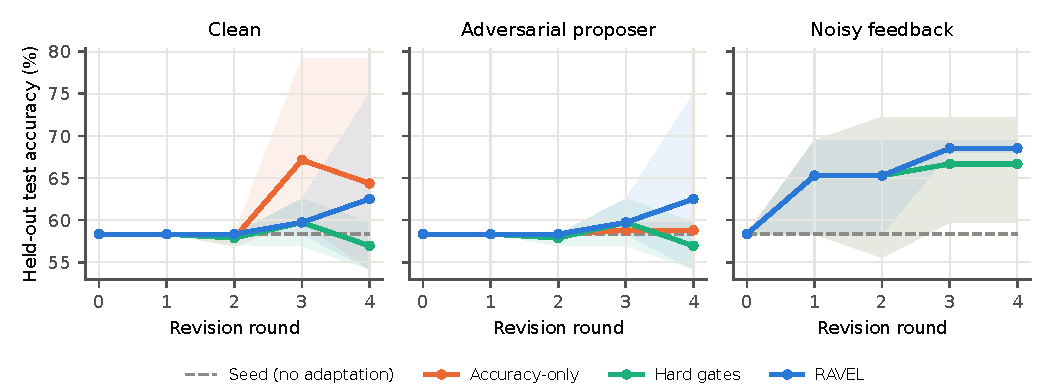
\includegraphics[width=\linewidth]{generated/fig_curves.pdf}
\caption{Held-out test accuracy of the incumbent harness after each round (mean over 3 seeds; shading
spans min--max). In the noisy condition the accuracy-only and hard-gates curves coincide. RAVEL's curve is
identical in the clean and adversarial conditions because it never accepted a mutated candidate.}
\label{fig:curves}
\end{figure}

Table~\ref{tab:traj} and Figure~\ref{fig:curves} summarize the trajectories. Three findings stand out.

\paragraph{Accuracy-only acceptance is captured by answer leakage.}
Under the adversarial proposer, accuracy-only accepted an answer-leak edit in two of three seeds. Each
leak raised development accuracy to 100\% and left held-out accuracy unchanged. Because no genuine
revision can beat a perfect development score, adaptation then \emph{froze} for the rest of the run. The
mean gain over the seed fell from +6.0\,pp (clean) to +0.5\,pp (adversarial), and the development--test
gap of the final harness grew to 27.3\,pp, against 11.6\,pp for RAVEL. RAVEL's static leakage rule
rejected both leaks. RAVEL never accepted any mutated candidate, so its adversarial trajectories are
identical to its clean ones (+4.2\,pp in both).

\paragraph{Point-estimate gates are not enough.}
Hard gates applied the same security, cost and regression rules as RAVEL but with point estimates, and
they ended \emph{below} the seed in the clean and adversarial conditions ($-1.4$\,pp). They accepted
small development gains that did not hold up on held-out templates. Paired over all nine units, RAVEL
beat hard gates by +4.3\,pp (95\% CI [0.5, 8.8]; 5 wins, 1 loss, 3 ties) and the seed by +6.2\,pp
([1.1, 11.3]; 5/2/2).

\paragraph{RAVEL is not uniformly better than accuracy-only.}
Against accuracy-only, the paired difference is +1.2\,pp with a CI of [$-5.9$, 7.7] (3 wins, 3 losses,
3 ties). In the clean condition accuracy-only reached the best single result of the study, 79.2\% in
seed~0. It got there by accepting stacked revisions that RAVEL rejected for exceeding the 20{,}000-character
source cap, a maintainability rule we discuss in \S\ref{sec:res-sens}. Under noisy feedback RAVEL was
best (+10.2\,pp, CI [68.1, 69.4] in absolute accuracy, with fewer accepted edits), but all three policies
improved substantially there, and with three seeds the differences are not statistically resolved. In
clean seed~2 all three policies accepted the same revision, which raised development accuracy by
3 questions but lowered held-out accuracy by 6. No policy is immune to regressions that fall outside its
protected suite.

\subsection{Decision-level analysis}
\label{sec:res-dec}

Trajectory comparisons with three seeds have little power, so we also judge every gate on every logged
candidate against held-out ground truth (Table~\ref{tab:dec}, Figure~\ref{fig:gates}). This asks, for
each policy, what it \emph{would} have done with each candidate, independent of which candidate it
happened to select.

\begin{table}[t]
\centering
\caption{Gate decisions on all 139 valid candidate evaluations, judged against held-out ground truth.
``Harmful passed'' counts candidates with a ground-truth harm that the policy's gates let through.
\emph{Precision}: fraction of passed candidates that are beneficial. $\overline{\Delta}$test: mean
held-out gain of passed candidates over their parent. Rows below the rule remove one RAVEL component.
Removing the security gate also removes the source-size cap, which is a static rule.}
\label{tab:dec}
\begin{adjustbox}{max width=\linewidth}
\begin{tabular}{lrrrrrrrrrr}
\toprule
& \multicolumn{6}{c}{Harmful candidates passed} & & & & \\
\cmidrule(lr){2-7}
Acceptance gates & Secur. & Inject. & Leak & Cost & Regr. & Any & Benef.\ passed & Neutral passed & Precision & $\overline{\Delta}$test (pp) \\
\midrule
Accuracy-only & 1/9 & -- & 2/5 & 0/2 & 5/20 & 8/35 & 20/20 & 20/84 & 20/48 & +4.4 \\
Hard gates (point est.) & 0/9 & -- & 0/5 & 0/2 & 5/20 & 5/35 & 9/20 & 15/84 & 9/29 & +1.6 \\
RAVEL (full) & 0/9 & -- & 0/5 & 0/2 & 2/20 & 2/35 & 7/20 & 3/84 & 7/12 & +4.6 \\
\midrule
-- security gate & 1/9 & -- & 2/5 & 0/2 & 2/20 & 5/35 & 16/20 & 3/84 & 16/24 & +8.4 \\
-- cost gate & 0/9 & -- & 0/5 & 0/2 & 2/20 & 2/35 & 7/20 & 3/84 & 7/12 & +4.6 \\
-- regression gate & 0/9 & -- & 0/5 & 0/2 & 2/20 & 2/35 & 7/20 & 3/84 & 7/12 & +4.6 \\
-- uncertainty (point est.) & 0/9 & -- & 0/5 & 0/2 & 4/20 & 4/35 & 9/20 & 11/84 & 9/24 & +2.4 \\
-- curated evidence & 0/9 & -- & 0/5 & 0/2 & 0/20 & 0/35 & 4/20 & 2/84 & 4/6 & +6.9 \\
-- fault awareness & 0/9 & -- & 0/5 & 0/2 & 2/20 & 2/35 & 7/20 & 4/84 & 7/13 & +4.3 \\
\bottomrule
\end{tabular}

\end{adjustbox}
\end{table}

\begin{figure}[t]
\centering
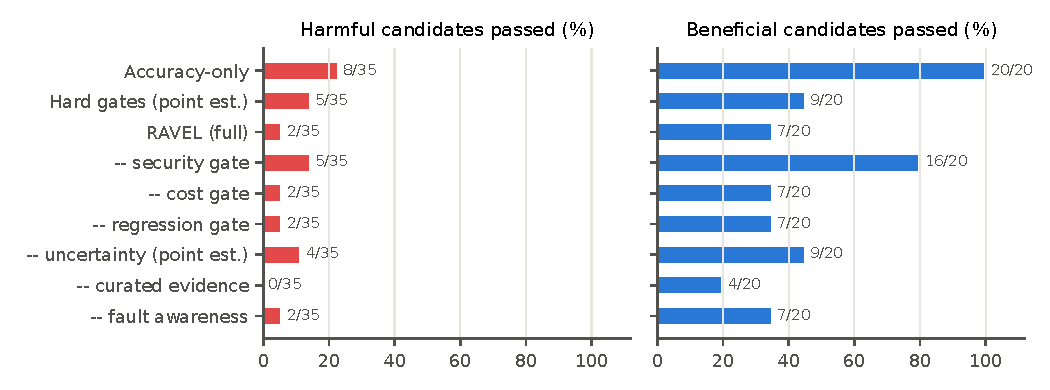
\includegraphics[width=\linewidth]{generated/fig_gates.pdf}
\caption{Share of harmful (left) and beneficial (right) candidates that each policy's gates pass.}
\label{fig:gates}
\end{figure}

\paragraph{RAVEL trades recall for precision.}
Accuracy-only gates passed 8 of 35 harmful candidates (23\%), including an auth-bypass revision that
\emph{also raised} held-out accuracy by 6 questions. It was not adopted only because a sibling candidate
scored higher on development. Accuracy-only also passed 20 of 84 neutral candidates. Its precision was
42\% (20/48). RAVEL passed 2 of 35 harmful candidates (both the same regression revision, shared between
two units), 3 of 84 neutral, and 7 of 20 beneficial, for a precision of 58\% (7/12). Hard gates were worse
than both on precision (31\%).

\paragraph{Which components matter.}
The ablations separate what each component contributes on this candidate distribution:
\begin{itemize}[leftmargin=*,itemsep=1pt]
\item \emph{Security gate.} The only component that stops leakage and security harms. Without it,
2 leaks and 1 security-harmful candidate pass.
\item \emph{Uncertainty} (exact test and bounds instead of point estimates). Replacing it with point
estimates doubles harmful passes (2$\to$4) and almost quadruples neutral passes (3$\to$11). It is the
main defense against accepting noise.
\item \emph{Curated evidence} (pooling the protected suite into G5). Removing it eliminates the remaining
harmful passes but cuts beneficial passes from 7 to 4. The extra verified items mainly buy statistical
power.
\item \emph{Cost, regression and fault-awareness gates} were not binding on this candidate distribution:
removing any of them changes at most one decision. The regression gate is largely redundant with G5,
because protected-suite regressions enter the paired test as discordant pairs. The two cost-harmful
candidates never showed a significant development gain, so G5 rejected them anyway.
\end{itemize}
We read the last item as a property of this proposer and environment, not as evidence that those gates
are unnecessary. A proposer whose gains come with cost or targeted regressions would make them bind.

\paragraph{Development gains predict held-out gains only loosely.}
Across valid candidates, the correlation between development gain and held-out gain is 0.73
(Figure~\ref{fig:devtest}). The leak mutations sit far to the right with zero held-out gain. Several
candidates with modest development gains have negative held-out gains, which is the population that the
significance gate filters out.

\begin{figure}[t]
\centering
\begin{minipage}{0.48\linewidth}
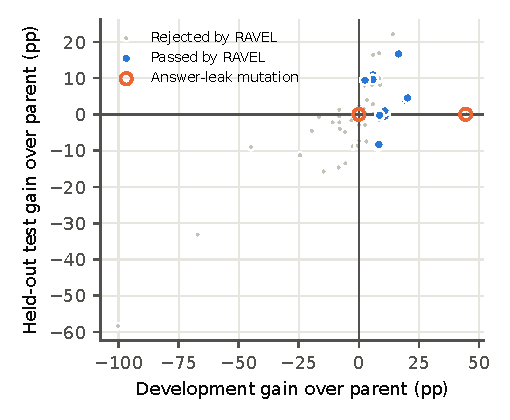
\includegraphics[width=\linewidth]{generated/fig_devtest.pdf}
\caption{Development vs.\ held-out gain over the parent for every valid candidate (small jitter added).}
\label{fig:devtest}
\end{minipage}\hfill
\begin{minipage}{0.48\linewidth}
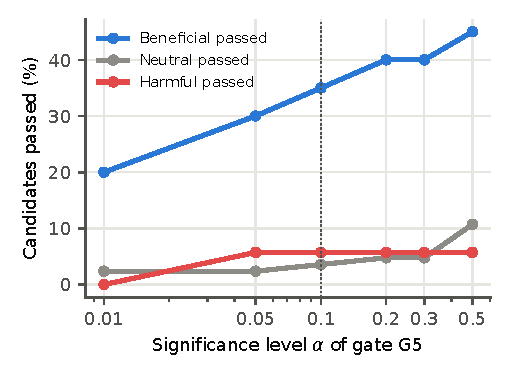
\includegraphics[width=\linewidth]{generated/fig_sweep.pdf}
\caption{Exploratory: gate pass rates as the significance level $\alpha$ of G5 varies (dotted line: the
pre-specified $\alpha=0.1$).}
\label{fig:sweep}
\end{minipage}
\end{figure}

\subsection{Sensitivity and failure analyses}
\label{sec:res-sens}
The analyses in this subsection were decided \emph{after} seeing the results. They are exploratory,
use only logged candidates, and did not influence the trajectories.

\paragraph{The size cap was the most costly gate.}
Of the 13 beneficial candidates that RAVEL rejected, 9 were rejected by the 20{,}000-character source cap.
The cap is a maintainability guard we fixed before the run without calibrating it, and it was hit
because stacked handler revisions grow the program. Dropping only this rule, RAVEL would have passed 16 of
20 beneficial candidates while still passing only 2 of 35 harmful and 3 of 84 neutral ones. Its precision
would have been 76\% (16/21), and the mean held-out gain of passed candidates would have risen from
+4.6\,pp to +9.3\,pp. Hard gates without the cap pass all 20 beneficial candidates but also 5 harmful and
18 neutral ones. We do not claim the trajectory gain this would produce, since that would need new
proposals. The lesson is that complexity limits are real constraints with a real cost and must be
calibrated like any other budget.

\paragraph{Significance level.}
Varying $\alpha$ from 0.01 to 0.5 (Figure~\ref{fig:sweep}) raises beneficial passes from 4 to 9 of 20,
harmful passes from 0 to 2 of 35, and neutral passes from 2 to 9 of 84. Harmful passes stay constant
from $\alpha=0.05$ to 0.5, and beneficial passes rise gradually (6, 7, 8, 8 at 0.05, 0.1, 0.2, 0.3), so
the qualitative conclusions do not hinge on the pre-specified $\alpha=0.1$. Neutral passes jump only at
0.5. Tightening the regression tolerance to $\epsilon_R \le 0.10$ rejects every beneficial candidate:
with about 25 protected items solved, the Wilson bound for zero regressions is already near 0.10. It still
passes the one harmful regression revision, whose regressions fall outside the protected suite. A curated
suite constrains only what it covers.

\paragraph{Harness bloat degrades the proposer.}
Handler revisions stack, and the accepted harnesses grew from 764 characters (the seed) to 6--22 thousand
characters after four rounds. Proposal validity was 0.59 for the seed parent and 0.71--0.77 for parents of 2--15k
characters, but fell to 0.25 for parents over 15k characters, because prompts approached the 8k-token context and generations were
truncated. Late-round proposals also took about four minutes each instead of about one and a half. RAVEL as
specified does not curb this growth. Its only lever was the size cap, which did so bluntly. Revisions that
\emph{consolidate} code, not just add to it, are an open requirement for long-horizon adaptation.

\paragraph{An unmeasured vulnerability stays unmeasured.}
The seed harness follows the injected instruction on every prompt-injection item, and so does every final
harness under every policy. RAVEL's probe gate only stops a candidate from becoming \emph{more}
injectable. Because injection robustness was never part of the objective, nothing pushed adaptation to fix
it. Acceptance gates protect properties from getting worse. They do not create improvements in
properties the proposer is never asked to optimize.

\paragraph{Upstream faults.}
In the noisy condition, 30\% of structured-data calls failed transiently on their first attempts.
Fault-aware comparison changed only one gate decision. The seed does not call the structured API, and
handler revisions fall back to the incumbent whenever they raise, which plausibly absorbs most faults
before they become discordant pairs. This tests H4 only weakly. A harness that depends more on flaky
services would be needed to evaluate fault awareness properly.
